\documentclass[12pt]{article}

\usepackage[spanish,activeacute]{babel}
\usepackage[utf8]{inputenc}
\usepackage{graphicx}
\usepackage{amsmath}
\usepackage{listings}
\usepackage[usenames,dvipsnames]{color}
%\usepackage{fullpage}

\lstdefinestyle{mycode} 
{language=C++, basicstyle=\small,frame=tb,rulecolor=\color{blue},aboveskip=0.35cm,belowskip=0.35cm,commentstyle=\color{gray20}}


\title{Ocultar datos en archivos de sonido}
\author{Juan Antonio Cano Salado \and Borja Moreno Fernández \and Pascual Javier Ruiz Benítez}

\begin{document}

\maketitle

\newpage
\tableofcontents

\newpage
\section{Resumen}

Este trabajo aborda la ocultación de datos en archivos de sonido o, lo que es lo mismo, la esteganografía de audio. El objetivo de esta disciplina consiste básicamente en ocultar información (de cualquier tipo) en archivos de sonido, de forma que los cambios llevados a cabo en el archivo original resulten imperceptibles para una persona.

Comenzaremos estudiando los principios básicos de la esteganografía en general, y de la esteganografía de audio en particular. A continuación, analizaremos algunos de los métodos más comúnmente utilizados en esteganografía de audio. Hecho esto, estudiaremos uno de los formatos de audio más populares: el formato WAV. Finalmente, incluiremos una descripción de la implementación realizada y proporcionaremos un manual de instalación y manejo de la aplicación desarrollada.

\section{Introducción}

\subsection{Esteganografía}

La esteganografía es la disciplina en la que se estudian y aplican técnicas que permiten el ocultamiento de mensajes u objetos, dentro de otros, llamados portadores, de modo que no se perciba su existencia.

Los orígenes de la esteganografía datan de la antigua Grecia. Heródoto, famoso historiador griego, informa del uso de la esteganografía en informes de Grecia a Persia. El método consistía en afeitar la cabeza de un esclavo y tatuar allí un mensaje. Dicho mensaje quedaba oculto cuando el pelo del esclavo volvía a crecer. Para leer el mensaje sólo era necesario volver a afeitarle la cabeza al esclavo. La idea era que nadie sospechase de la existencia de dicho mensaje.

La esteganografía ha sido usada en numerosas ocasiones a lo largo de la historia: tintas invisibles, acrósticos o mensajes microscópicos son sólo algunas de sus formas. Recientemente, en plena era digital, la estaganografía ha adquirido gran importancia como tecnología utilizada en el campo de la seguridad informática. Pueden ocultarse mensajes secretos en correos electrónicos, imágenes, audio e incluso vídeo.

Diversos grupos han mostrado tener un gran interés en las aplicaciones de la esteganografía. Algunos, interesados en la protección de derechos de autor. Otros, preocupados por proteger la privacidad de sus mensajes. Muchos gobiernos temen que la esteganografía podría convertirse en una herramienta de gran utilidad para criminales y grupos terroristas. En cualquier caso, parece claro que existen multitud de aplicaciones y usos para la esteganografía, y la mayoría de los expertos están de acuerdo en que será un tema de gran interés durante los próximos años.

La figura \ref{prisioneros} ilustra un ejemplo simple de un problema en el que el uso de la esteganografía puede ser de utilidad.

\begin{figure}[h]
  \centering
    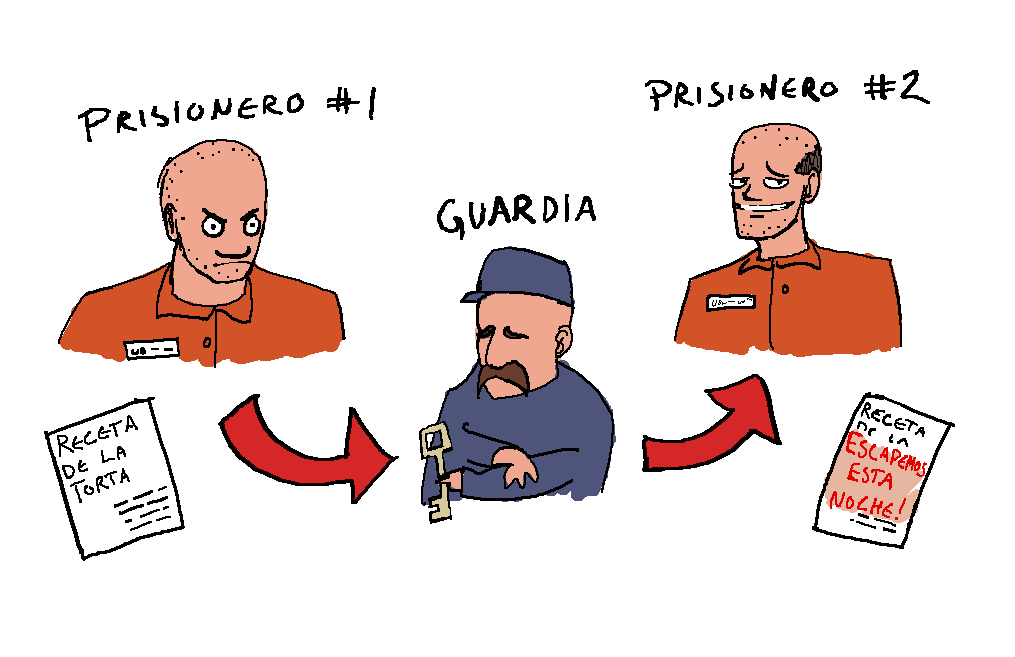
\includegraphics[width=\textwidth]{img/illustration2}
  \caption{Problema de los prisioneros}
  \label{prisioneros}
\end{figure}

Dos prisioneros en una cárcel necesitan comunicarse para ultimar los detalles de un plan de fuga, pero tienen un gran problema: el guardia de la prisión tiene acceso a toda la correspondencia entre los prisioneros. La criptografía por sí sola no es una solución. Un mensaje cifrado levantaría todo tipo de sospechas. Los prisioneros deben idear un sistema que les permita pasar mensajes de apariencia inocente, con información oculta que sólo ellos puedan entender. Esto es exactamente lo que persigue la esteganografía.

La esteganografía puede además combinarse con la criptografía para crear sistemas más seguros. Así, distinguimos:

\begin{itemize}

\item Esteganografía pura

La fortaleza del sistema recae en los algoritmos de ocultación y extracción de la información, que solo el emisor y el receptor del mensaje deberían conocer.

\item Esteganografía de clave privada

Fruto de la combinación de esteganografía pura con criptosistemas simétricos. Se asume que un atacante podría conocer los algoritmos de ocultación y extracción de la información. Por este motivo, el mensaje se cifra utilizando un cifrado simétrico antes de ocultarlo. De esta manera, incluso si el atacante intercepta la transmisión y logra extraer la información aún tendrá que enfrentarse al criptoanálisis del criptosistema utilizado.

\item Esteganografía de clave pública

Basada en unir esteganografía pura y criptosistemas de clave pública. De esta manera, el emisor y el receptor evitan tener que compartir una clave privada.

\end{itemize}

\subsection{Audio digital}

El audio digital se diferencia del sonido analógico tradicional en que es una señal discreta en lugar de una señal continua. Esta señal discreta es creada llevando a cabo un proceso de muestreo y cuantización de una señal analógica continua. La frecuencia de muestro varía según los propósitos. Por ejemplo, la frecuencia de muestreo estándar para un CD de audio digital es de alrededor de 44kHz. La figura \ref{audiodigital} ilustra el proceso de muestro y cuantización para producir una señal de audio digital a partir de una señal continua de audio analógico.
En dicha figura se ha exagerado la naturaleza discreta de la señal digital. Sin embargo, las frecuencias de muestreo usuales permiten que el audio digital sea prácticamente idéntico a la señal de audio analógica original.

\begin{figure}[h]
  \centering
    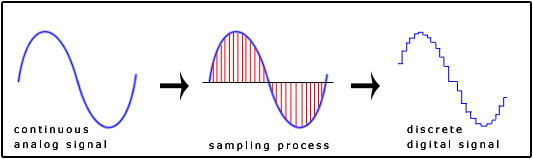
\includegraphics[width=\textwidth]{img/digitalaudio}
  \caption{Audio digital}
  \label{audiodigital}
\end{figure}

Los archivos de audio digital se almacenan en el ordenador como una secuencia de ceros y unos. Con las herramientas apropiadas, es posible alterar individualmente los bits que componen estos archivos. Esto hará posible llevar a cabo modificaciones a la secuencia binaria que produzcan cambios en la señal de audio que no sean perceptibles al oído humano.

\subsubsection{El formato WAV}

WAV (o WAVE), apócope de WAVEform audio file format, es un formato de audio digital normalmente sin compresión de datos desarrollado y propiedad de Microsoft y de IBM que se utiliza para almacenar sonidos en el PC. Admite archivos mono y estéreo a diversas resoluciones y velocidades de muestreo. Su extensión es .wav.

Es una variante del formato RIFF (Resource Interchange File Format, formato de fichero para intercambio de recursos). El formato toma en cuenta algunas peculiaridades de la CPU Intel, y es el formato principal usado por Windows.
A pesar de que el formato WAV es compatible con casi cualquier códec de audio, se utiliza principalmente con el formato PCM (no comprimido) y, al no tener pérdida de calidad, es adecuado para uso profesional. Para tener calidad CD de audio se necesita que el sonido se grabe a 44100 Hz y a 16 bits. Por cada minuto de grabación de sonido se consumen unos 10 megabytes de espacio en disco. Una de sus grandes limitaciones es que solo se pueden grabar archivos de 4 gigabytes como máximo, lo cual equivale aproximadamente a 6,6 horas en calidad de CD de audio. Es una limitación propia del formato, independientemente de que el sistema operativo donde se utilice sea MS Windows u otro distinto, y se debe a que en la cabecera del fichero se indica la longitud del mismo con un número entero de 32 bits.

En Internet no es popular, fundamentalmente porque los archivos sin compresión son muy grandes. Son más frecuentes los formatos comprimidos con pérdida, como el MP3 o el Ogg Vorbis. Como éstos son más pequeños, la transferencia a través de Internet es mucho más rápida. Además, existen códecs de compresión sin pérdida más eficaces, como Apple Lossless o FLAC.

Estudiaremos este formato debido a su sencillez. Será además el formato empleado por la aplicación desarrollada (véase sección ``Implementación realizada'').

Los archivos RIFF comienzan con una cabecera seguida de una secuencia de chunks de datos (fragmentos de información). Los archivos WAVE son archivos RIFF con un único chunk llamado ``WAVE'' que se divide en dos sub-chunks:

\begin{itemize}

\item fmt

Especifica el formato de los datos.

\item data

Contiene la información de sonido dividida en samples (porciones de audio).

\end{itemize}

La figura \ref{wavsoundformat} muestra gráficamente la organización de un archivo WAV de audio digital. Podemos observar la división en tres partes claramente diferenciadas (RIFF, fmt y data) así como los campos que componen cada una de ellas (incluyendo tamaño, nombre, posición relativa en el archivo, etc.). En conjunto, la cabecera del archivo (compuesta por RIFF, fmt, y parte de data) tiene un tamaño de 44 bytes. Tras esta cabecera se encontraría la información de sonido real. A continuación ofrecemos una pequeña descripción de cada uno de los campos que componen esta cabecera.

\begin{figure}
  \centering
    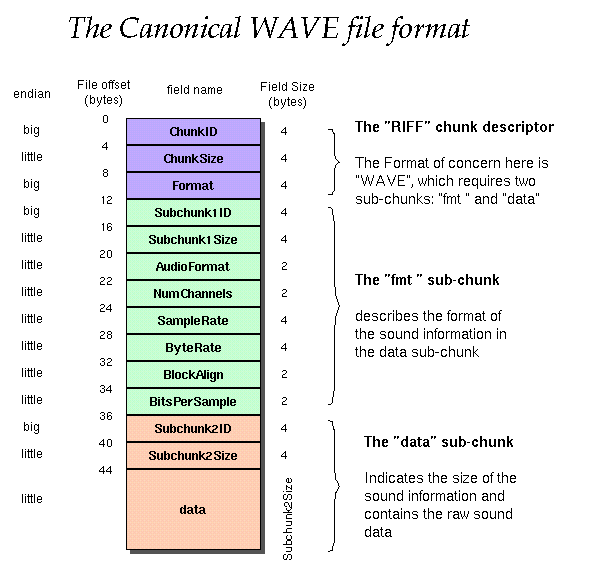
\includegraphics[width=\textwidth]{img/wavsoundformat}
  \caption{Formato WAV}
  \label{wavsoundformat}
\end{figure}

\begin{itemize}

\item ChunkID          

Contiene las letras ``RIFF'' en formato ASCII.

\item ChunkSize

36 + SubChunk2Size, o, más detallado:
4 + (8 + SubChunk1Size) + (8 + SubChunk2Size)
                               
Es el tamaño del archivo a partir de este punto. Es decir, el tamaño total del archivo menos los 8 bytes ya tratados (campos ChunkID y ChunkSize).

\item Format

Contiene las letras ``WAVE''.

\item Subchunk1ID

Contiene las letras ``fmt ''.

\item Subchunk1Size

16 en caso de usar PCM. Es el tamaño del resto de la sección ``fmt''.

\item AudioFormat

1 para PCM. Otros valores para otros tipos de compresión.

\item NumChannels

Número de canales. Mono = 1, Stereo = 2, etc.

\item SampleRate

Frecuencia de muestreo. 8000, 44100, etc.

\item ByteRate

SampleRate * NumChannels * BitsPerSample/8

\item BlockAlign

NumChannels * BitsPerSample/8
                               
El número de bytes para cada sample incluyendo todos los canales.

\item BitsPerSample

8 bits = 8, 16 bits = 16, etc.

\item Subchunk2ID

Contiene las letras ``data''.

\item Subchunk2Size

NumSamples * NumChannels * BitsPerSample/8
                               
Número de bytes de datos.

\item Data

Los datos de sonido.

\end{itemize}

\section{Descripción del problema}

En un sistema de estaganografía de audio, se ocultan mensajes secretos en audio digital. El mensaje secreto se introduce alterando ligeramente la secuencia binaria del archivo de audio. Existen aplicaciones de esteganografía de audio que permiten ocultar mensajes en archivos de audio en formato WAV, AU e incluso MP3.

Ocultar mensajes secretos en archivos de sonido suele ser más difícil que ocultar mensajes en archivos de imagen o vídeo. Esto se debe a la mayor sensibilidad que presenta en las personas el sistema auditivo frente al sistema visual. Existen un buen número de métodos y algoritmos para llevar a la práctica estos conceptos, algunos de ellos sencillos y otros más complejos (basados en técnicas avanzadas de procesado digital de señales). Estos métodos serán analizados en mayor detalle en la sección ``Soluciones presentadas".

\section{Soluciones presentadas}

En esta sección presentamos algunos de los métodos más comúnmente utilizados en esteganografía de audio. Pueden encontrarse implementaciones de estos métodos en la Web. Algunos de los métodos más avanzados requieren conocimiento previo de técnicas de procesado de señales, análisis de Fourier y otras áreas matemáticas. Se han preferido utilizar diagramas y pseudocódigo en lugar de fórmulas matemáticas exactas para intentar hacer la teoría más accesible a lectores con conocimientos básicos de esteganografía.

\subsection{Codificación en el bit menos significativo (LSB coding)}

Es el método más simple de inclusión de información en un archivo de audio digital. Se basa en sustituir el bit menos significativo de cada sample (porción de sonido) con un bit del mensaje a ocultar. Este método permite ocultar grandes cantidades de información. La figura \ref{lsbcoding} ilustra cómo se oculta el mensaje ``HEY'' en un archivo de audio compuesto por samples de 16 bits.

\begin{figure}
  \centering
    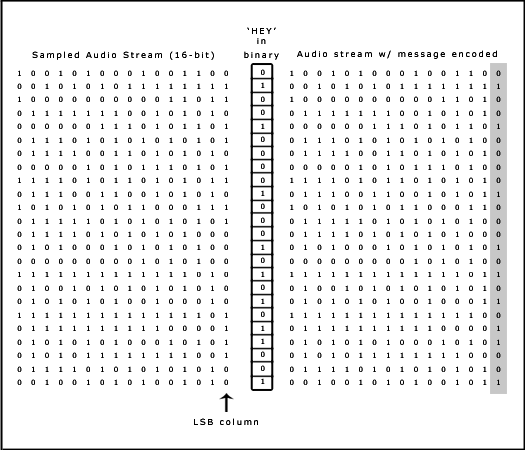
\includegraphics[width=\textwidth]{img/lsbimage}
  \caption{LSB Coding}
  \label{lsbcoding}
\end{figure}

Algunas implementaciones de este método utilizan los dos (o más) bits menos significativos de cada sample para ocultar información. Esto hace que la cantidad de información que se puede insertar aumente, pero también eleva la cantidad de ruido que es introducida en la señal de audio resultante. Por ello, es importante considerar el tipo de señal de audio antes de decidir el número de bits por sample a utilizar. Por ejemplo, un archivo de sonido grabado en una estación de metro con gran cantidad de ruido de fondo podría soportar la inclusión de dos o más bits de información en cada sample, ya que el ruido de fondo enmascararía el ruido introducido en el proceso de ocultación de información. Por contra, un archivo de sonido que contenga un solo de piano será mucho más sensible a estas modificaciones, por lo que el uso de más de un bit por sample podría hacer que las modificaciones resultaran perceptibles al oído humano.

Para poder extraer un mensaje secreto codificado utilizando LSB, el receptor necesita tener acceso a la secuencia de samples utilizada en el proceso de inserción de información. Normalmente, la longitud del mensaje secreto a ocultar es mucho menor que el número total de samples del archivo de sonido. Una decisión a tomar consiste por tanto en cómo elegir qué subconjunto de samples del archivo original se usarán para contener información. El emisor y el receptor deben ponerse de acuerdo en esta cuestión. Una técnica trivial consiste en comenzar en el inicio del archivo de sonido y llevar a cabo la inserción de información en los primeros samples, hasta que el mensaje ha sido completamente introducido. A partir de ahí, el resto de samples quedarían inalterados. El problema de esta técnica radica en que la primera parte del archivo de sonido tendrá propiedades estadísticas diferentes a la del resto del archivo, que no fue modificado. Una solución a este problema es añadir al mensaje secreto una secuencia de bits aleatorio de manera que la longitud total del mensaje fuera igual al número total de samples. El inconveniente es que el proceso de inserción modificaría ahora muchos más samples de los que la transmisión del mensaje original requería, lo cual hace que sea más sencillo detectar la existencia del mensaje oculto.

Una solución más sofisticada se basa en usar un generador de números pseudoaleatorios para distribuir el mensaje entre los samples del archivo de sonido. Para poder hacer esto, el emisor y el receptor deben ponerse de acuerdo en la semilla que utilizarán para generar la secuencia pseudoaleatoria de samples a utilizar. De esta manera el receptor puede reconstruir la secuencia y averiguar cuáles son los samples que contienen el mensaje oculto. Hay que tener cuidado con que el generador produzca el mismo sample dos veces. Si esto ocurriese, se modificaría el bit menos significativo de un sample cuyos bits menos significativos ya habían sido modificados, produciéndose una colisión. Una manera de evitar esto es almacenar en una lista los samples que ya han sido modificados, de manera que si el generador indica que se vuelva a utilizar un sample ya empleado, se ignora. Otra alternativa consiste en calcular una permutación pseudoaleatoria del conjunto de samples del archivo de audio, y seleccionar los primeros. Con esta técnica es imposible que se utilice el mismo sample más de una vez.

\subsection{Codificación en paridad (Parity Coding)}

En lugar de dividir la señal en samples individuales, este método divide la señal en regiones disjuntas. Una región es un conjunto de samples, de un tamaño determinado. Todas las regiones tendrán el mismo tamaño, excepto quizás la última, si el número de samples del archivo no es múltiplo del número de samples por región. El método oculta un bit del mensaje secreto en el bit de paridad de cada región. El bit de paridad de una región se define como el resultado de aplicar la operación lógica XOR a todos los bits de todos los samples de la región. Si el bit de paridad de la región seleccionada (aquella en la que se ha decidido ocultar un bit del mensaje) no coincide con el bit secreto a incrustar, se modifica el bit menos significativo de uno de los samples de la región (no importa cual). Si coincide, no es necesario llevar a cabo ninguna modificación. De esta manera, el emisor tiene una serie de samples entre los que elegir a la hora de ocultar cada bit.

\begin{figure}
  \centering
    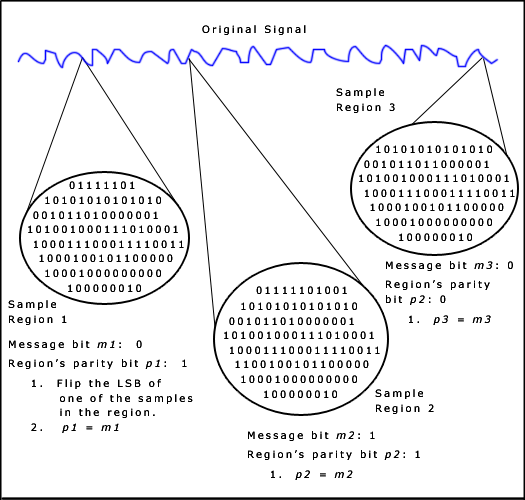
\includegraphics[width=\textwidth]{img/parity}
  \caption{Parity Coding}
  \label{paritycoding}
\end{figure}

La figura \ref{paritycoding} ilustra cómo se ocultan, usando este método, los tres primeros bits del mensaje ``HEY'' (010, ya que en formato ASCII la `H'\space se representa por el número 72 en decimal, 01001000 en binario).

Para poder llevar a cabo el proceso de extracción de la información el receptor debe conocer el tamaño de las regiones así como el orden en el que éstas fueron utilizadas a la hora de ocultar la información. Como en el método anterior, puede optarse por utilizar las primeras regiones del archivo de sonido de manera secuencial, o bien por usar un generador pseudoaleatorio que, a partir de una semilla, determine el orden en que deben escogerse las regiones en las que ocultar información. En caso de utilizar esta segunda alternativa, la semilla y el generador pseudoaleatorio deben ser compartidos por emisor y receptor, evidentemente.

El proceso de obtención de la información oculta se limita a calcular los bits de paridad de las regiones empleadas durante el proceso de inserción del mensaje. La concatenación de estos bits de paridad dará como resultado el mensaje original. Como puede observarse, el receptor no necesita conocer en ningún momento qué samples concretos se han visto modificados con respecto al archivo de sonido original.

\bigskip

Los métodos de codificación en el bit menos significativo y codificación de paridad presentan dos desventajas fundamentales. En primer lugar, ambos introducen ruido en la señal original, y el oído humano es muy sensible al ruido, a menudo siendo capaz de detectar incluso las cantidades más insignificantes. El método de codificación de paridad es ligeramente mejor en este aspecto, ya que asegura que sólo se modificará como máximo un bit en cada región. La otra gran desventaja que presentan estos métodos es que no son robustos. Pequeñas modificaciones en el archivo de sonido que contiene el mensaje secreto podrían destruir dicho mensaje. La robustez de estos métodos puede aumentar en cierta medida si se utilizan técnicas de redundancia, ocultando cada bit del mensaje secreto en dos o más localizaciones del archivo de audio. El problema que presenta esta solución es que aumenta la cantidad de bits a incrustar en el archivo de sonido original, lo cual reduce el tamaño máximo del mensaje que se puede ocultar en una señal de audio determinada a la vez que se incrementa la probabilidad de que las modificaciones realizadas resulten perceptibles.

\subsection{Codificación en fase (Phase coding)}

A diferencia de los métodos anteriores, el método de codificación en fase no está basado en la inserción de ruido y por tanto no comparte los inconvenientes previamente señalados. La idea centra en codificación en fase es que las componentes de fase del sonido no resultan tan perceptibles al oído humano como el ruido. Por ello, en lugar de introducir perturbaciones, esta técnica codifica los bits del mensaje como desplazamientos de fase en el espectro de fases de la señal digital.

\begin{figure}
  \centering
    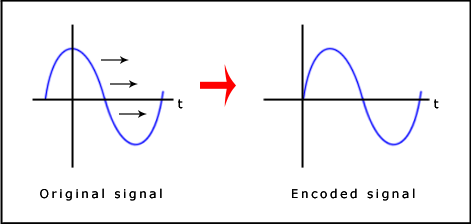
\includegraphics[width=\textwidth]{img/phaseshift}
  \caption{Phase Coding}
  \label{phasecoding}
\end{figure}

El procedimiento es el siguiente:

\begin{enumerate}

\item La señal de sonido original se divide en segmentos cuya longitud es igual al tamaño del mensaje a ocultar.

\item Se aplica la transformada discreta de Fourier a cada segmento para crear una matriz de las fases y magnitudes de la transformada de Fourier.

\item Se calculan las diferencias de fase entre segmentos adyacentes.

\item Desplazamientos de fase entre segmentos consecutivos serían fácilmente detectables. En otras palabras, las fases absolutas de los segmentos pueden cambiarse pero las diferencias relativas de fase entre segmentos adyacentes deben preservarse. Por este motivo, el mensaje secreto sólo se inserta en el vector de fases del primer segmento de la señal, de manera que la nueva fase será:

\[
\text{nueva\_fase }=\left\{
\begin{array}{ccc}
\pi /2 & \text{si} & \text{bit del mensaje = 0} \\
&  &  \\
-\pi /2 & \text{si} & \text{bit del mensaje = 1}
\end{array}
\right.
\]

\item Se crea una nueva matriz de fases usando las nuevas fases del primer segmento y respetando las diferencias de fase originales.

\item Usando la nueva matriz de fases y la matriz de magnitudes original, se reconstruye la señal de sonido aplicando la transformada discreta de Fourier inversa, y después concatenando los segmentos.

\end{enumerate}

Para extraer el mensaje secreto del archivo de sonido, el receptor debe conocer la longitud del segmento. Entonces puede usar la transformada discreta de Fourier para obtener las fases y extraer la información.

\medskip

Una desventaja del método de codificación en fase es su baja tasa de transferencia de información, debida al hecho de que el mensaje secreto sólo se codifica en el primer segmento de la señal. Este inconveniente podría mitigarse aumentando la longitud de los segmentos de la señal. Sin embargo, esto haría que las relaciones de fase entre cada componente de frecuencia cambiase de manera más drástica, haciendo más sencillo detectar la existencia del mensaje oculto. Por tanto, el método de codificación en fase se usa cuando sólo es necesario transmitir una pequeña cantidad de datos.

\subsection{Espectro ensanchado (Spread spectrum)}

En el contexto de la esteganografía de audio, el método básico de ensanchado del espectro intenta expandir la información secreta lo máximo posible en el espectro de frecuencia de la señal de audio. Esto es análogo a un sistema de codificación en el bit menos significativo en el que el mensaje se ocultara en bits elegidos aleatoriamente de entre todos los bits del archivo de sonido. Sin embargo, a diferencia de lo que ocurre en LSB coding, el método de espectro ensanchado distribuye los bits del mensaje secreto en el espectro de frecuencia del archivo de sonido, usando un código que es independiente de la señal. Como resultado, la señal final ocupa un ancho de banda mayor al originalmente requerido para la transmisión.

Se pueden usar dos versiones del método de espectro ensanchado en esteganografía de audio: el esquema de secuencia directa y el esquema de salto de frecuencia. En secuencia directa, el mensaje secreto se distribuye utilizando una constante llamada ``chip rate'' y luego se modula con una señal pseudoaleatoria. Después se entrelaza con la señal original. En salto de frecuencia, el espectro de frecuencia del archivo de audio es alterado para que salte rápidamente entre frecuencias.

La teoría matemática en la que se basa este método es bastante complicada y va más allá de los objetivos de este proyecto. El diagrama de la figura \ref{spreadspectrum} ilustra el diseño de un sistema de esteganografía de audio basado en espectro ensanchado utilizando el esquema de secuencia directa.

\begin{figure}
  \centering
    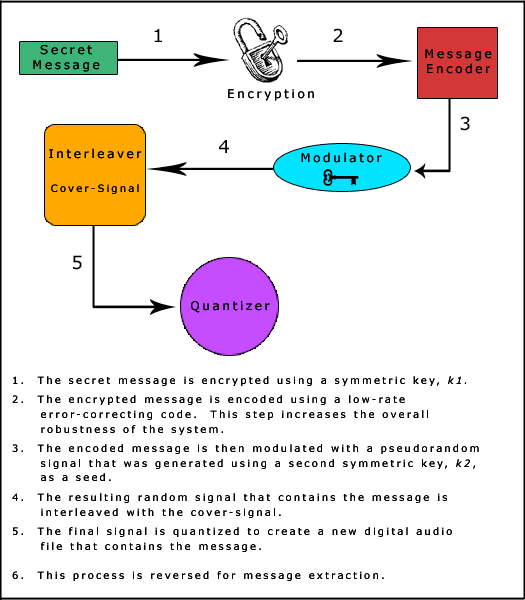
\includegraphics[width=\textwidth]{img/spreadspectrum}
  \caption{Spread Spectrum}
  \label{spreadspectrum}
\end{figure}

El método de espectro ensanchado ofrece una tasa de transmisión de datos moderada y un nivel de robustez alto (más alto que el obtenido con cualquiera de los métodos anteriores). Sin embargo, comparte una desventaja con los métodos de codificación en el bit menos significativo y codificación en paridad: introduce ruido en el archivo de sonido.

\subsection{Ocultamiento en eco (Echo hiding)}

En este método la información es insertada en el archivo de sonido introduciendo un eco en la señal discreta. Como el método de espectro ensanchado, ofrece una tasa de transmisión de datos alta y proporciona una robustez elevada.

Para ocultar la información con éxito, se utilizan tres parámetros del eco: amplitud, decadencia y offset (retraso) de la señal original. Todos estos parámetros se establecen en valores inferiores al umbral de perceptibilidad que marca el oído humano. El offset varía según el bit del mensaje original a insertar. Un valor de offset representa el uno binario y un segundo valor de offset representa el cero binario.

\begin{figure}
  \centering
    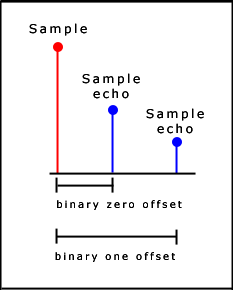
\includegraphics[width=0.5\textwidth]{img/echooffsets}
  \caption{Offsets del eco}
  \label{echooffsets}
\end{figure}

Si sólo se produjera un eco a partir de la señal original, sólo podría insertarse un bit de información. Por ello, la señal original se divide en bloques antes de que comience el proceso de inserción de información. Una vez que el proceso termina, los bloques son concatenados para crear la señal de audio final.

A continuación describiremos una versión sencilla del método de ocultamiento de eco. Dividiremos la señal completa en bloques, aunque en circunstancias normales debería dejarse un número aleatorio de samples sin usar entre cada par de bloques, para reducir la probabilidad de detección.

En primer lugar la señal se divide en bloques, y a cada bloque se le asigna un uno o un cero en función del mensaje secreto a ocultar. En nuestro ejemplo, el mensaje será la secuencia binaria asociada a `HEY' (véase figura \ref{echodividesignal}).

\begin{figure}
  \centering
    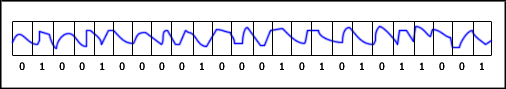
\includegraphics[width=\textwidth]{img/echodividesignal}
  \caption{Señal dividida en bloques y bit asociado a cada bloque}
  \label{echodividesignal}
\end{figure}

A continuación se usa el siguiente algoritmo (se muestra pseudocódigo) para insertar la información necesaria en cada bloque:

\begin{lstlisting}[style=mycode]
init(Block blocks[]) { 
   for (int i=0; i < blocks.length; i++) { 
      if (blocks[i].echoValue() == 0) 
         blocks[i] = offset0(blocks[i]); 
      else 
         blocks[i] = offset1(blocks[i]); 
   } 
}
Block offset0(Block block) { 
   return (block + (block - OFFSET_0)); 
}

Block offset1(Block block) { 
   return (block + (block - OFFSET_1)); 
}
\end{lstlisting}

Por último, los bloques se recombinan para producir la señal final.

Usar la implementación descrita del proceso de ocultación de eco usualmente resultará en una señal con una mezcla de ecos considerable, lo que incrementa el riesgo de detección. Describimos ahora una segunda implementación que intenta solventar este problema. Primero se crea una señal de eco de la señal original completa utilizando el offset asociado al cero binario. Luego generamos una segunda señal de eco asociada a la señal original global, usando el valor de offset asociado al uno binario. La señal ``uno'' sólo contiene unos, y la señal ``cero'' sólo contiene ceros. Para combinar las dos señales de eco y conseguir la señal final, se usan dos señales de mezcla. Las señales de mezcla tienen un valor de uno o cero, según el bit a insertar en el bloque. En nuestro ejemplo, para ocultar el mensaje ``HEY'' obtendríamos las señales de mezcla mostradas en la figura \ref{mixersignals}.

\begin{figure}
  \centering
    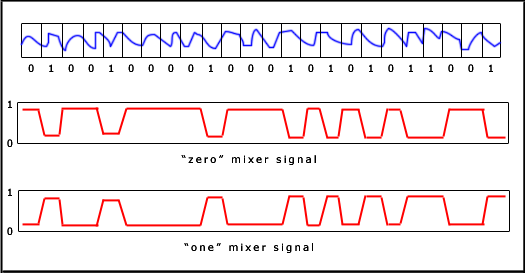
\includegraphics[width=\textwidth]{img/mixersignals}
  \caption{Señales de mezcla}
  \label{mixersignals}
\end{figure}

La señal de eco ``uno'' se multiplica por la señal de mezcla ``uno'' y la señal de eco ``cero'' se multiplica por la señal de mezcla ``cero''. Hecho esto, las dos señales resultantes se suman para obtener la señal final. La señal final obtenida utilizando este procedimiento es menos abrupta que la obtenida usando el primer procedimiento descrito. Esto se debe a que las dos señales de mezcla son complementarias y a que se usan transiciones lineales suaves.

El diagrama de la figura \ref{echo2ndimp} resume esta segunda implementación del método de ocultamiento en eco.

\begin{figure}
  \centering
    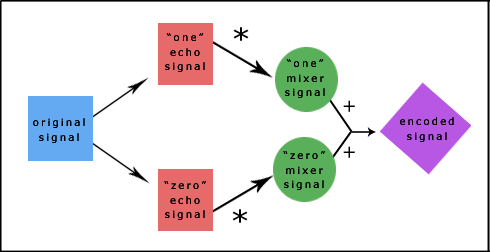
\includegraphics[width=\textwidth]{img/echo2ndimp}
  \caption{Ocultamiento en eco: segundo procedimiento}
  \label{echo2ndimp}
\end{figure}

Para extraer el mensaje secreto, el receptor debe ser capaz de dividir la señal en el mismo conjunto de bloques usado durante el proceso de inserción de la información. Hecho esto, puede usarse la función de autocorrelación del cepstrum de la señal (el cepstrum es la transformada de Fourier del espectro de frecuencias de la señal) para extraer el mensaje, ya que ésta muestra un pico en cada offset de eco en el tiempo, lo que permite reconstruir el mensaje.

\section{Conclusiones}

La esteganografía de audio es muy flexible y esto es lo que la hace tan interesante. Los cinco métodos analizados dan a los usuarios gran capacidad de decisión y hacen la tecnología accesible a un gran número de personas. A la hora de escoger qué método de esteganografía de audio emplear, debe estudiarse la importancia de factores como la tasa de transferencia de datos, el ancho de banda, la robustez y la perceptibilidad, para elegir el método que mejor se ajuste a las necesidades. Por ejemplo, dos personas que sólo necesitan enviarse un mensaje secreto ocasionalmente podrían usar el método de codificación en el bit menos significativo, fácil de implementar. Por contra, una gran multinacional con la intención de proteger su propiedad intelectual de ``piratas digitales'' probablemente consideraría métodos más sofisticados como codificación en fase, espectro ensanchado u ocultamiento de eco. Otro de los aspectos de la esteganografía de audio que la hace tan atractiva es su capacidad para combinarse con las tecnologías de criptografía ya existentes. Los usuarios no tienen que elegir cuál de los dos métodos utilizar, la información puede ir cifrada y oculta simultáneamente.

En resumen, con el crecimiento de áreas como protección de copyright, protección de privacidad y vigilancia, creemos que la esteganografía seguirá aumentando en importancia. La esteganografía de audio, en particular, se centra en problemas que se originaron con la aparición del audio digital (y su espectacular auge con el formato MP3), el software P2P, y la necesidad de un esquema de comunicaciones seguro que pueda mantener el secreto de la información transmitida incluso si ésta debe atravesar canales inseguros.

\section{Problemas abiertos}

\section{Implementación realizada}

\section{Manual de instalación y manejo de la aplicación}

\section{Bibliografía}

\section{Tabla de tiempos}

\end{document}